\section{Approach}
\label{sec:appr}

This section describes problems with using \unsafe{} that we identified, as well as information on how to exploit these issues in the wild.
Furthermore, we present our two novel tools, \toolUsage{} and \toolSA{}, that aid in locating, evaluating and fixing potentially dangerous \unsafe{} usages in source code.


%% ---------------------------------------------------

\subsection{Usage and Security Problems}

In the following, we discuss potential threat models and exploit vectors against real-world \unsafe{} Go code.
We present a code pattern in Listing~\ref{lst:string-to-bytes} that is very common in popular open-source Go projects (cf. Section~\ref{sec:eval}).
It is used to convert a string to a byte slice and vice versa without copying the data.
As in Go strings essentially are just read-only byte slices, this is commonly done by projects to increase efficiency of serialization operations. % and is possible as in Go, strings are essentially read-only byte slices.
Internally, each slice is represented by a data structure that contains its current length, allocated capacity, and memory address of the actual underlying data array.
The \texttt{reflect} header structures provide access to this internal representation.
In Listing~\ref{lst:string-to-bytes} this conversion is done in line 2, 3, and 8 respectively.
First, an \texttt{unsafe.Pointer} is used to convert a \texttt{string} to a \texttt{reflect.StringHeader} type.
Then, a \texttt{reflect.SliceHeader} instance is created and its fields are filled by copying the respective values from the string header.
Finally, the slice header object is converted into a slice of type \texttt{[]byte}.

\begin{lstlisting}[language=Golang, label=lst:string-to-bytes, caption=Conversion from string to bytes using \unsafe{}, float, belowskip=-1.5em]
func StringToBytes(s string) []byte {
	strHeader := (*reflect.StringHeader)(unsafe.Pointer(&s))
	bytesHeader := reflect.SliceHeader{
		Data: strHeader.Data,
		Cap:  strHeader.Len,
		Len:  strHeader.Len,
	}
	return *(*[]byte)(unsafe.Pointer(&bytesHeader))
}
\end{lstlisting}


\subsubsection*{Implicit Read-Only}

The conversion pattern shown in Listing~\ref{lst:string-to-bytes} is efficient as it directly casts between \texttt{string} and \texttt{[]byte} in-place, without the need to reallocate the slice.
Using \texttt{bytes := ([]byte)(s)} for the conversion would make the compiler allocate new memory for the slice header as well as the underlying data array.
However, this pattern creates an implicitly read-only byte slice that can cause problems later on, as described in the following.

The Go compiler will place strings into a constant data section of the resulting binary file.
Therefore, when the binary is loaded into memory the \texttt{Data} field of the string header may contain an address that is located on a read-only memory page.
Because of this, strings are immutable by design in Go.
Mutating a string will cause a compiler error, alerting developers early in the development process that there is a problem.
However, when casting the string to a \texttt{[]byte} slice in-place, the resulting slice loses the explicit read-only property, and thus, the compiler will not complain about mutating this slice although the program will crash if done so.
Using this pattern, therefore, creates a trade-off between performance and potentially hard-to-find bugs that can lead to crashes.
%Due to the indirection resulting from the conversion to a slice which gets then passed around, they can be very hard to debug.


\subsubsection*{Garbage Collector Race}

Go uses a concurrent mark-and-sweep garbage collector to free unused memory~\cite{sibiryov2017}.
It is triggered either by a certain increase of heap memory usage or after a fixed time, and runs in multiple parallel threads (Goroutines).
The garbage collector treats pointer types, \texttt{unsafe.Pointer} values, and slice/string headers that belong to actual slices/strings as references and will mark them as still in use. %, preventing them from being freed.
Importantly, string or slice headers that are created manually as well as \texttt{uintptr} values are not treated as references.
The last point, although documented in the \texttt{unsafe} package, is a major pitfall.
Casting an \texttt{uintptr} variable back to a pointer type creates a potentially dangling pointer because the memory at that address might have already been freed if the garbage collector was triggered right before the conversion.

Although not directly obvious, Listing~\ref{lst:string-to-bytes} contains such a condition.
Because the \texttt{reflect.SliceHeader} value is created as a composite literal instead of being derived from an actual slice value, its \texttt{Data} field is not treated as a reference if the garbage collector runs between lines 3 and 8. 
Thus, the underlying data array of the \texttt{[]byte} slice produced by the conversion might have already been collected.
This creates a potential \textit{use-after-free} or buffer reuse condition that, even worse, is triggered non-deterministically when the garbage collector runs at just the "right" time.
If the buffer is reused after being freed and the slice resulting from the cast is pointing to it, it can provide access to completely unrelated data. % even in concurrent Goroutines. 
Therefore, this race condition can crash the program, create an information leak, or even potentially lead to code execution.
Figure~\ref{fig:gcrace-vuln} shows a visualization of the casting process that leads to the problems described here.
The original slice is being cast to a string via some intermediate representations.
The slice header is shown in green (at memory position 1), while the underlying data array (memory position 2) is shown in red.
When the resulting string header (shown in blue at memory position 3) is created, it only has a weak reference to the data, and when the garbage collector runs before converting it to the final string value, the data is already freed.

\begin{figure}[!t]
    \vspace{2mm}
    \centering
    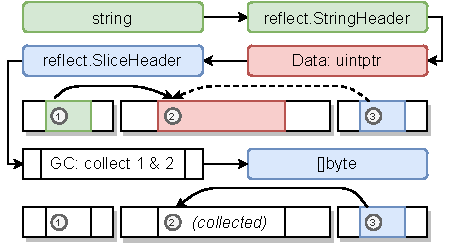
\includegraphics[width=0.4\textwidth]{gfx/figures/gcrace-vuln.pdf}
    %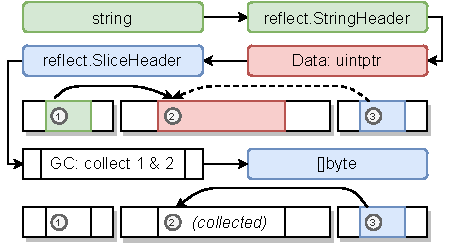
\includegraphics[width=0.48\textwidth]{gfx/figures/gcrace-vuln.pdf}
    \caption{GC race and escape analysis flaw}
    \label{fig:gcrace-vuln}
    \vspace{-8pt}
\end{figure}



\subsubsection*{Escape Analysis Flaw}

A third problem with the casting pattern shown in Listing~\ref{lst:string-to-bytes} is that the escape analysis algorithm can not infer a connection between the string parameter \texttt{s} and the resulting byte slice.
Although they use the same underlying data array, the algorithm misses this due to the fact that the intermediate representation as \texttt{uintptr} variable is not treated as a reference type.
This can cause undefined behavior if the returned value from the casting function is used incorrectly.

Listing~\ref{lst:escape-analysis} shows a simple program that uses the common conversion function presented earlier in Listing~\ref{lst:string-to-bytes}.
In the \texttt{main} function, \texttt{GetBytes} is called (Line 2) which creates a string and converts it into a byte slice using an \unsafe{} cast.
Within the function \texttt{GetBytes}, we create the string using a \texttt{bufio} reader similarly to if it were user-provided input.
After the cast, \texttt{GetBytes} prints the resulting bytes (Line 10) and returns them back to \texttt{main}, which also prints the bytes (Line~3).
Although, one might assume that both print statements result in the same string to be displayed, the second one in \texttt{main} fails and prints invalid data.


% // expected (but failed) stdout is "abcdefgh
% // expected stdout is "abcdefgh"
\begin{lstlisting}[language=Golang, label=lst:escape-analysis, caption=Escape analysis flaw example, float, belowskip=-1.5em]
func main() {
	bytesResult := GetBytes()
	fmt.Printf("main: %s\n", bytesResult)
}

func GetBytes() []byte {
	reader := bufio.NewReader(strings.NewReader("abcdefgh"))
	s, _ := reader.ReadString('\n')
	out := StringToBytes(s)
	fmt.Printf("GetBytes: %s\n", out)
	return out
}
\end{lstlisting}

This happens because when the string \texttt{s} is allocated in \texttt{GetBytes}, Go escape analysis will be triggered. %try to figure out if it escapes.
It concludes that \texttt{s} is passed to \texttt{StringToBytes} and the escape analysis transitively looks into that function, where it fails to connect \texttt{s} to the returned byte slice as described previously.
Therefore, the escape analysis finds that \texttt{s} does not escape in \texttt{StringToBytes} 
As it is not used after the call in \texttt{GetBytes}, the algorithm incorrectly assumes that it does not escape at all and places \texttt{s} on the stack.
When \texttt{GetBytes} prints the resulting slice, the data is still valid and the correct data is printed, but once the function returns to \texttt{main}, its stack is destroyed.
Thus, \texttt{bytesResult} (Line~2) is now a dangling pointer into the former stack of \texttt{GetBytes} and, therefore, printing data from an invalid memory region.


%\subsubsection*{Correct In-Place Cast}
%
%To avoid the problems described in the previous sections, it is crucial to not create instances of \texttt{reflect.SliceHeader} and \texttt{reflect.StringHeader} from scratch, instead they must be derived from actual slices or strings.
%Although this is documented with the \texttt{unsafe} package, there are many incorrect usages in the projects we analyzed.
%A correct version of the in-place cast is shown in Listing~\ref{lst:correct-slice-cast}.
%
%\begin{lstlisting}[language=Golang, label=lst:correct-slice-cast, caption=Correct in-place string to bytes cast]
%func StringToBytes(s string) (b []byte) {
%	strHeader := (*reflect.StringHeader)(unsafe.Pointer(&s))
%	bytesHeader := (*reflect.SliceHeader)(unsafe.Pointer(&b))
%	bytesHeader.Data = strHeader.Data
%	bytesHeader.Cap = strHeader.Len
 %   bytesHeader.Len = strHeader.Len
%	return
%}
%\end{lstlisting}


\subsubsection*{Potential Code Execution}

To show the severity of the issues identified above and that they are not just of theoretical nature, e.g., resulting in simple program crashes, we created a proof of concept for a code execution exploit using Return Oriented Programming (ROP) on a vulnerability caused by a misuse of \unsafe{}.
This vulnerability causes a buffer overflow, and since Go programs are typically statically linked with a big runtime, ASLR is not effective as there are a large number of ROP-gadgets available.
An in-depth discussion of the exploit would go beyond the scope of this paper and exceed the space available to present our research.
Therefore, we made the proof-of-concept code available online with other related exploit demonstrations in a public repository\footnote{\url{https://github.com/jlauinger/go-unsafepointer-poc}}. 


%% ---------------------------------------------------

\subsection{\toolSA{}: An Unsafe-focused Linter for Developers}

This section presents \toolSA{}, a novel static code analysis tool to find dangerous \unsafe{} usage patterns that were previously uncaught with existing tools.
All source code for \toolSA{} is made publicly available\footnote{\url{https://github.com/jlauinger/go-safer}}.

\subsubsection*{Design}

Figure~\ref{fig:safer-architecture} shows an overview of the architecture of \toolSA{}.
It was built on top of the existing infrastructure provided by the \textit{go vet} tool.
First, \textit{go vet} builds a list of packages to be analyzed from the user input and parses the sources of those packages.
Then, a number of static code analyzers, called \textit{passes}, run.
We depend on existing passes to acquire the abstract syntax tree (AST) and control flow graph (CFG) for our analyses.
\toolSA{} runs two separate analysis passes: the \textit{sliceheader} pass discovers incorrect string and slice casts as shown in Listing~\ref{lst:string-to-bytes}.
The \textit{structcast} pass finds unsafe casts between different struct types that include architecture-dependent field sizes and, therefore, might create a security risk when ported to other platforms.
Describing potential exploit vectors for this second type of problem is beyond the scope of this paper, thus, we added an example of this to the public repository mentioned in the last section.

\begin{figure}[!t]
    \vspace{2mm}
    \centering
    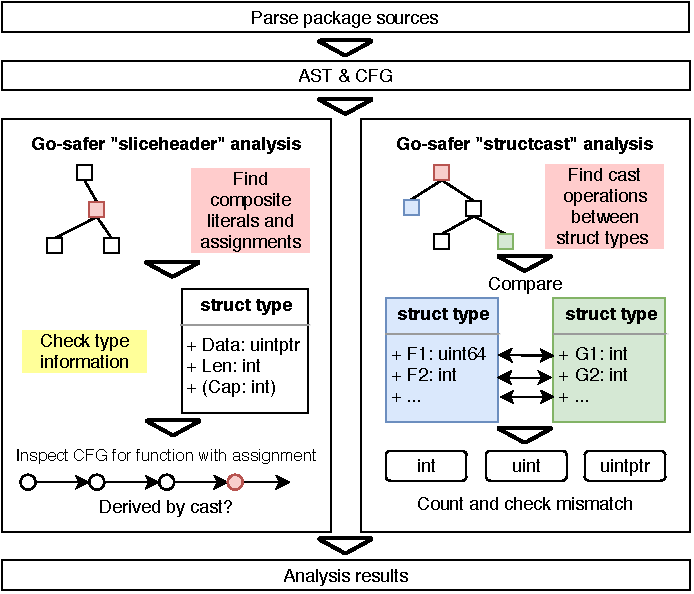
\includegraphics[width=0.48\textwidth]{gfx/figures/go-safer-architecture.pdf}
    %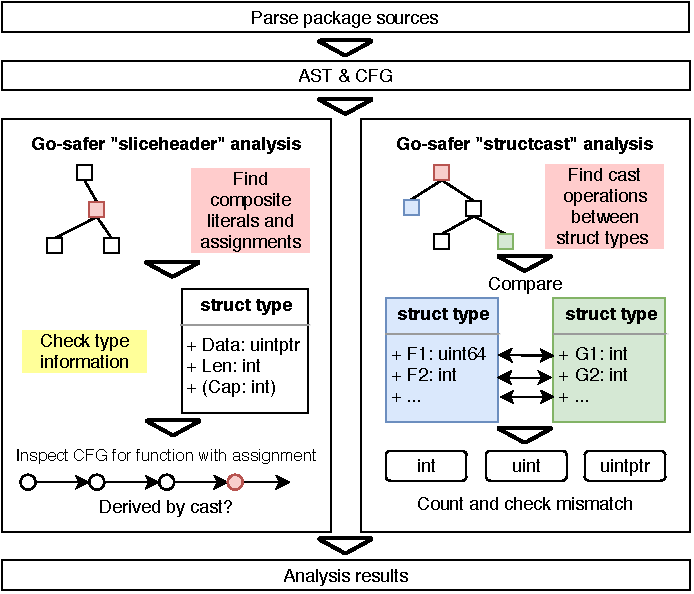
\includegraphics[width=0.45\textwidth]{gfx/figures/go-safer-architecture.pdf}
    \caption{Architecture of \toolSA{} static code analysis tool}
    \label{fig:safer-architecture}
    %\vspace{-14pt}
\end{figure}


%% put this here to manually position the figure one page earlier. Belongs to the next section (go-geiger), reposition if needed.
\begin{figure}[htp!]
    %\vspace{2mm}
    \centering
    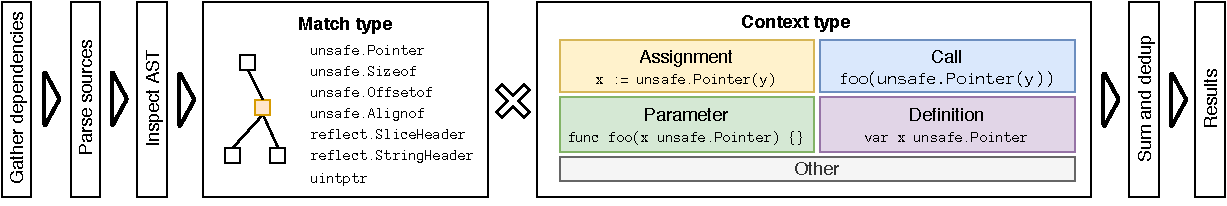
\includegraphics[width=\textwidth]{assets/figures/chapter4/go-geiger-architecture.pdf}
    \caption{Architecture of the \toolGeiger{} tool to detect unsafe usages}
    \label{fig:geiger-architecture}
    %\vspace{-10pt}
\end{figure}



\subsubsection*{Implementation}

The \textit{sliceheader} pass finds composite literals and assignment statements in the AST.
Then, for each of them it checks whether the type of the %literal or assignment 
receiver is \texttt{reflect.StringHeader}, \texttt{reflect.SliceHeader}, or some derived type with the same signature.
For assignments, the analysis pass then finds the last node in the CFG where the receiver object's value is defined, and checks if is derived correctly by casting a string/slice.
If \toolSA{} can not infer with certainty that the assignment receiver object was created by a cast, then \toolSA{} issues a warning.

The \textit{structcast} pass finds instances of in-place casts between different struct types using an intermediate representation as \texttt{unsafe.Pointer}.
Then, it compares the struct types and checks if they contain an unequal amount of fields with types \texttt{int}, \texttt{uint}, or \texttt{uintptr}, which are the architecture-dependent types supported by Go.
If the numbers do not match, \toolSA{} issues a warning.


%% ---------------------------------------------------

\subsection{\toolUsage{}: Automatic Identification of Unsafe Usage}

This section presents \toolUsage{}, a novel tool to identify and quantify usages of \unsafe{} in a package and its dependencies.
The \toolUsage{} tool is also available on GitHub\footnote{\url{https://github.com/jlauinger/go-geiger}}.
Its development was inspired by \textit{cargo geiger}\footnote{\url{https://github.com/rust-secure-code/cargo-geiger}}, a similar tool for detecting unsafe code blocks in Rust programs.

\subsubsection*{Design}

Figure~\ref{fig:geiger-architecture} shows an overview of the architecture of \toolUsage{}.
We use the standard parsing infrastructure provided by Go to identify and parse packages including their dependencies based on user input.
%In particular, we use the \texttt{packages.Load} function to parse the sources of all packages requested for analysis including their transitive dependencies.
Then, we analyze the AST %using the standard \texttt{ast.Inspect} function.
which enables us to identify different usages of \unsafe{} and their context as described in the next paragraph.
Finally, we arrange the packages requested for analysis and their dependencies in a dependency tree and sum up \unsafe{} usages for each package individually as well a cumulative score including dependencies.
We also perform a deduplication if the same package is transitively imported more than once.
The \unsafe{} dependency tree, usage counts, as well as identified code snippets, are then presented to the user.

\subsubsection*{Implementation}

We detect all usages of methods and fields from the \texttt{unsafe} package, specifically: \texttt{Pointer}, \texttt{Sizeof}, \texttt{Offsetof}, and \texttt{Alignof}.
Furthermore, because they often are used in unsafe operations, we also count occurrences of \texttt{reflect.SliceHeader}, \texttt{reflect.StringHeader}, and \texttt{uintptr}.
All of these usages are referred to as \unsafe{} usages in this paper.

The first six \unsafe{} types are detected by finding selector expression nodes with matching field names, while \texttt{uintptr} usages are found by inspecting identifier nodes in the AST.
Additionally, we determine the context in which the \unsafe{} usage is found.
Context here means the type of statement that includes the \unsafe{} usage.
In \toolUsage{} we distinguish between assignments (including definitions of composite literals and return statements), calls to a function, function parameter declarations, general variable definitions, or other not further specified usages.
We determine the context by looking up in the AST starting from the node representing the \unsafe{} usage, and identifying the type of a parent node.
%For example, if the nearest relevant ancestor in the AST is an \texttt{AssignStmt} node, then the context is determined as assignment.
